\chapter{Cálculo del Ch del S\&H}

El tiempo necesario para la cuantificación y la codificación de señales depende de la resolución deseada, del método de conversión y de la velocidad de los componentes empleados. Por otra parte, la velocidad con que se debe convertir una señal depende de sus variaciones temporales y de la exactitud deseada. Pero no sólo deber ser el CAD suficientemente rápido de acuerdo con el criterio Nyquist, sino que además debiera hacer la conversión de forma instantánea, pues de lo contrario se tiene una incertidumbre en la amplitud de la señal adquirida. Si la conversión dura un tiempo $t_c$, la salida obtenida corresponderá al valor de la señal en algún momento dentro de dicho intervalo de tiempo, pero no se sabe cuál. \par
\vspace{0.25cm}
Un amplificador de muestreo y retención soluciona este problema a base de tomar una muestra de la tensión de entrada y almacenarla en un condensador durante el tiempo que dure la conversión. De este modo no hace falta que la conversión sea muy rápida; basta que lo sea la adquisición de la muestra. La salida del CAD corresponde entonces al valor de la entrada en el "instante" de muestreo. El tiempo de conversión vendrá limitado solamente por el criterio de Nyquist. \par
\vspace{0.25cm}
Independientemente de los detalles del circuito o del tipo de S\&H en cuestión, todos estos dispositivos tienen cuatro componentes principales. El amplificador de entrada, el dispositivo de almacenamiento de energía (condensador), el búfer de salida y los circuitos de conmutación son comunes a todos los S\&H. En la figura \ref{fig:muestreo-retencion} se muestra la configuración típica del circuito de muestreo y retención.

\begin{figure}[H]
    \centering
    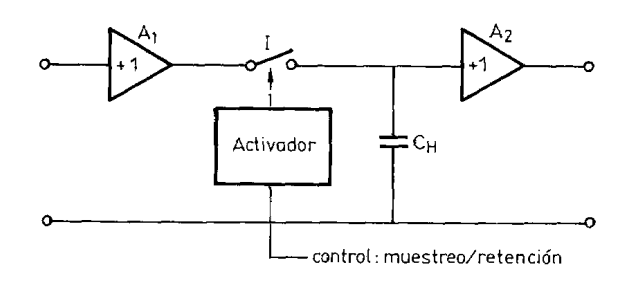
\includegraphics[width=0.5\linewidth]{Imagenes/S&H.png}
    \caption{Circuito de Muestreo y Retención (S\&H): Configuración Básica}
    \label{fig:muestreo-retencion}
\end{figure}

\section{Cálculo del condensador de holding $(C_h)$}
Si se elige un $C_h$ excesivamente pequeño, se cargará muy rápidamente pero podrá no retener la información suficiente tiempo. Si se elige un $C_h$ excesivamente grande, mantendrá la información durante bastante tiempo pero se tardará mucho en cargarlo con lo que podría incumplir el tiempo de asentamiento estipulado. La solución deberá estar entre dos valores ($C_{h, min}$ y $C_{h,max}$) que satisfagan ambos requisitos.

\begin{itemize}
    \item Cálculo de $C_{h, max}$. \\
    Si es demasiado grande podríamos incumplir el tiempo de asentamiento estipulado. La limitación está pues en el tiempo de asentamiento: hemos de garantizar que el condensador alcanza el valor final (menos el error permitido) durante el tiempo de asentamiento. \\
    De las condiciones de carga consideraremos la $I_{o, max}$ ya que las otras dos son menos relevantes y, en todo caso, se suponen minimizadas por el fabricante del S\&H. \\
    En consecuencia consideramos la carga de un condensador a corriente constante (mientras no se alcance el valor final se puede considerar el AO cortocircuitado y, por tanto, entregando la $I_{o, max}$ de cortocircuito.
    \[Q = I \times T = C \times C\]
    \[C = I \times \frac{T}{V}\]
    Donde: 
    \begin{itemize}
        \item $C$: $C_{h, max}$
        \item $I$: $I_{o, max}$
        \item $T$: $T_s$ (tiempo de asentamiento)
        \item $V$: $V_{fs}$ (tensión de fondo de escala)
    \end{itemize}

    \item Cálculo de $C_{h, min}$. \\
    La descarga del condensador se produce por las corrientes de fuga que podemos considerar constantes ($I_{fugas}$). \\
    El condensador deberá mantener el valor de la señal durante el tiempo de conversión ($T_c$) con un error no superior al permitido ($Err$). 
    \[C_{h, min} = I_{fugas} \frac{T_c}{Error}\]
    
\end{itemize}

Se elegirá un valor comprendido entre $C_{h, min}$ y $C_{h,max}$. Una vez elegido se comprobará que cumple con las otras condiciones.

\[C_{h, min} = I_{fugas} \frac{T_c}{Error}\]
\[C_{h, max} = I_{o, max} \frac{T_s}{V_{fs}}\]